50. $y=\sqrt{1+4x+4x^2}-3=|2x+1|-3=\begin{cases}2x+1-3=2x-2,\ x\geqslant-\cfrac{1}{2},\\ -2x-1-3=-2x-4,\ x<-\cfrac{1}{2}.\end{cases}$
$$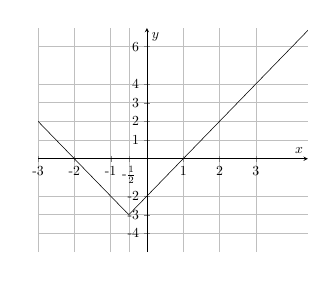
\begin{tikzpicture}[scale=0.5]
\begin{axis}[
    axis lines = middle,
    grid=major,
    legend pos={south west},
    xlabel = {$x$},
    ylabel = {$y$},
    ymin=-5,
    ymax=7,
    xtick={-3,-1,1,3,5,2,-2,-0.5},
    xticklabels={-3,-1,1,3,5,2,-2,-$\frac{1}{2}$},
    ytick={ 6, 2,-6, -2,1,4,-4,3,-3},
    yticklabels={ 6, 2,-6, -2,1,4,-4,3,-3}           ]
	\addplot[domain=-3:5, samples=100, color=black] {abs(1+2*x)-3};
%\addplot[domain=-3:5, samples=100, color=black] {-abs(x-1)};
%\addplot[domain=-3.1:2.5, samples=100, color=red] {70*abs(1-2*abs(abs(x)-2))-10*x^2+10*x-70};
	%\addlegendentry{$\text{Рис. 1}$};
\end{axis}
\end{tikzpicture}$$
